\documentclass{beamer}
\usetheme{Pittsburgh}
\usepackage{cmap}
\usepackage{graphicx}
\usepackage{listings}
\usepackage{microtype}
\lstset{escapeinside={<@}{@>}}
\setbeamertemplate{footline}[frame number]
\title{Una introducci\'on program\'atica a R en RStudio}
\author{\texorpdfstring{Diego Alburez Guti\'errez\newline\url{alburezg@lse.ac.uk}}{Diego Alburez Guti\'errez}}
\date{EncuestoEntusiastas - 2016}
\institute{London School of Economics}

\begin{document}

\begin{frame}
\maketitle
\end{frame}

\begin{frame}
\frametitle{Objetivos}
Al finalizar este taller, usted 
 \begin{enumerate}
  \item entender\'a la estructura b\'asica de R;
  \item podr\'a importar y manipular datos;
  \item sabr\'a c\'omo crear escribir c\'odigo reproducible en R
  \item Conocer\'a procedimientos para describir la desigualdad de ingresos; y
  \item tendr\'a una base s\'olida para seguir aprendiendo.
 \end{enumerate}
\end{frame}

\begin{frame}
\frametitle{Contenido}
\tableofcontents
\end{frame}

\section{D\'ia 1}

\begin{frame}
 \begin{center}
  \Huge \textcolor{blue}{D\'ia 1}
 \end{center}
\end{frame}

\subsection{Qu\'e es R y por qu\'e usarlo}
\frame{\tableofcontents[currentsection]}

  \begin{frame}{Qu\'e es R\footnote{https://www.r-project.org/about.html}}
R is an integrated suite of software facilities for data manipulation, calculation and graphical display.
     \begin{itemize}
		\item an effective data handling and storage facility,
		\item a suite of operators for calculations on arrays, in particular matrices,
		\item a large, coherent, integrated collection of intermediate tools for data analysis,
		\item graphical facilities for data analysis and display either on-screen or on hardcopy, and
		\item a well-developed, simple and effective programming language which includes conditionals, loops, user-defined recursive functions and input and output facilities.
      \end{itemize}
  \end{frame}
  
    \begin{frame}{Por qu\'e R}
     \begin{itemize}
     \item Gratuito	y colaborativo
          \begin{itemize}
               \item Stackoverflow 139,342 temas 
			   \item R-Bloggers
          \end{itemize}
      \item Popularidad creciente
      \item Usado en varias disciplinas (SPSS = Statistical Package for the Social Sciences)
	  \item En constante crecimiento
	  \item Archivos port\'atiles (.csv y .txt)
      \end{itemize}
  \end{frame}
  
\begin{frame}
      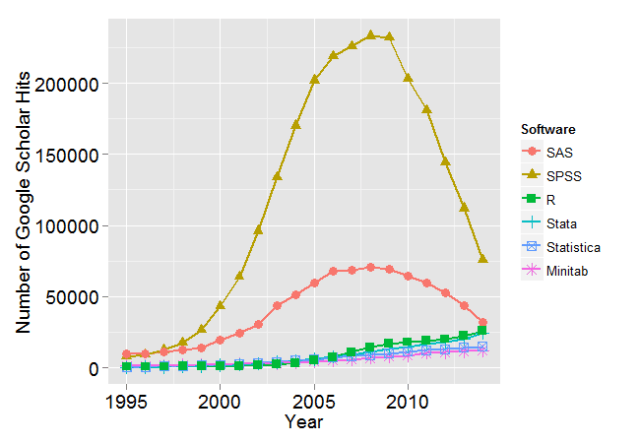
\includegraphics[scale=0.5]{use}\footnote{http://r4stats.com/articles/popularity/}
\end{frame}

\begin{frame}
      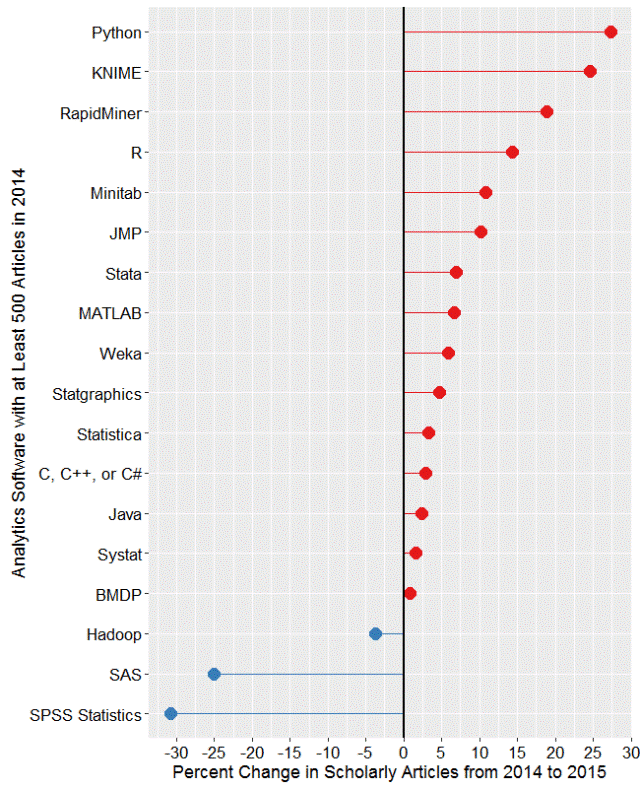
\includegraphics[scale=0.4]{change}\footnote{http://r4stats.com/articles/popularity/}
\end{frame}

\begin{frame}{Qu\'e puedo hacer con R}
     \begin{itemize}
	  \item Virtualmente cualquier an\'alisis estad\'istico
      \item An\'alisis reproducible
      \item Gr\'aficas
      \item Correr c\'odigo python, SQL, Stata, etc.
      \item Integrar con \LaTeX
      \item Generar reportes via \textcolor{blue}{\hyperlink{hhttp://rmarkdown.rstudio.com/}{markdown}}
     \end{itemize}
Adem\'as..
     \begin{itemize}
      \item Cualquier cosa: Lenguaje Turing completo
	  \item Aplicaciones web: \textcolor{blue}{\hyperlink{https://jschoeley.shinyapps.io/hmdexp/}{mortalidad}}, \textcolor{blue}{\hyperlink{https://haschke.shinyapps.io/PTS-App/}{terror}}
	  \item \textcolor{blue}{\hyperlink{rqda.r-forge.r-project.org/}{An\'alisis cualitativo}}, OCR, 'Cloud computing', etc.
      \end{itemize}
  \end{frame}

\begin{frame}{Im\'agenes para identificar ejes?}
      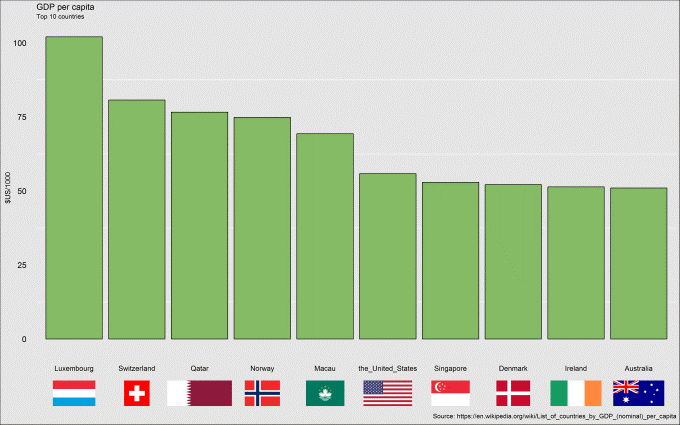
\includegraphics[scale=0.5]{imagen}
  \end{frame}

\begin{frame}{Mapas, etc}
      
\includegraphics[scale=0.5]{fb}
  \end{frame}
 
\begin{frame}{Pero...}
      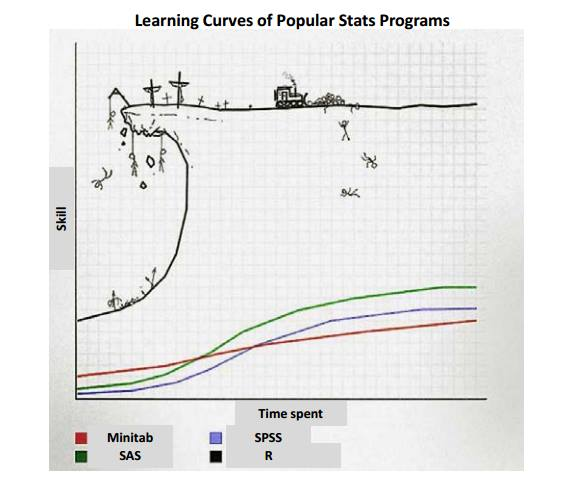
\includegraphics[scale=0.5]{learn}
\end{frame}
  
\subsection{RStudio: una interfaz de usuario para R}
\frame{\tableofcontents[currentsection]}

\begin{frame}{RStudio}
Principales elementos:
     \begin{itemize}
      \item L\'inea de comando
      \item Ventana de objetos/historial
      \item Visualizador
      \item Ventana para edici\'on de c\'odigo
     \end{itemize}
  \end{frame}

\subsection{Estructuras de datos en R}
\frame{\tableofcontents[currentsection]}

\defverbatim[colored]\lst{%
\begin{lstlisting}[language=R,tabsize=8,basicstyle=\ttfamily]
 x <- 42
 x
[1] 42
 y <- x
 y
[1] 42
 x + y
[1] 84
\end{lstlisting}
}

 \begin{frame}
 \frametitle{Operadores de asignaci\'on}
 Dos operadores casi an\'alogos:
      \begin{itemize}
 	    \item \textbf{$<$-} preferible por ahora
	    \item \textbf{=} (para asignar argumentos en una funci\'on)
  	   \end{itemize}
  	   \textcolor{blue}{Ejemplo}
\lst
\end{frame}

\defverbatim[colored]\lst{%
\begin{lstlisting}[language=R,tabsize=8,basicstyle=\ttfamily]
 x <- 6^2
 x
[1] 36
 x*4
[1] 144
y <- (x*4+6)/3
y
[1] ?
\end{lstlisting}
}

 \begin{frame}
 \frametitle{Operadores aritm\'eticos}
      \begin{itemize}
 	    \item \textbf{+}    Suma
	    \item \textbf{-}    Resta
	    \item \textbf{*}    Mult
	    \item \textbf{/}    Div
	    \item \textbf{\^{}} Expon
  	   \end{itemize}
  	   \textcolor{blue}{Ejemplo}
\lst
\end{frame}

\defverbatim[colored]\lst{%
\begin{lstlisting}[language=R,tabsize=8,basicstyle=\ttfamily]
 x <- 42
 x == 42
[1] TRUE
 x >= 6
[1] FALSE
 x = 6 <@\textcolor{red}{\# que hace esta linea?}@>
\end{lstlisting}
}

 \begin{frame}
 \frametitle{Operadores l\'ogicos}
      \begin{itemize}
 	    \item \textbf{$<$} menor que; \textbf{$>$} mayor que
 	    \item \textbf{$<$=} menor igual que; \textbf{$>$=} mayor igual que
 	    \item \textbf{==} igual a
 	    \item \textbf{!=} no es igual a
 	    \item \textbf{I} OR
 	    \item \textbf{\&} AND
  	   \end{itemize}
  	   \textcolor{blue}{Ejemplo}
\lst
\end{frame}

\begin{frame}{Tipos de objetos}
 \setbeamertemplate{enumerate items}[square]
     \begin{enumerate}
      \item Vectores
	  \item Matrices
	  \item Data frames
	  \item Operadores de referencia (ojo, estos no son objetos!)
	  \item Listas
	  \item Funciones
	  \item Paquetes
      \end{enumerate}
  \end{frame}

 \begin{frame}
 \frametitle{Vectores}
Contenedores de datos de menor nivel. Pueden ser:
      \begin{enumerate}
 	    \item Num\'ericos (numeric, integer); ej. 1 4 6
	    \item Caracteres (character); ej. "a" "b" "c"
	    \item L\'ogicos (logical); ej. TRUE FALSE
	    \item Fecha (date, POSIXt, ...); ej. "2009-09-15"
	    \item Categ\'oricos (factor) 
	    \item ...
  	   \end{enumerate}
  	   Recordar que:
  	   \begin{itemize}
  	   \item Cada vector puede albergar datos de un solo tipo
  	   \item Los vectores no pueden tener nombres num\'ericos ni incluir operadores (+,-,...)
  	   \item Los vectores no deben llamarse de la misma forma que funciones existentes.
  	   \item Usar el operador c() para crear vectores  con m\'as de un elemento. 
  	   \item Usar comillas ("") para asignar valores de texto
  	   \end{itemize}
\end{frame}

\defverbatim[colored]\lst{%
\begin{lstlisting}[language=R,tabsize=8,basicstyle=\ttfamily]
localidad <- c("urbano", "rural", NA, NA, 
           "rural")
localidad
[1] "urbano" "rural" NA NA "rural" 
<@\textcolor{red}{\# Se evaluan mediante el comando 'is.na()'}@>
is.na(localidad)
[1] FALSE FALSE  TRUE  TRUE FALSE
<@\textcolor{red}{\# Use '!' para evaluar la funcion opuesta:}@>
!is.na(localidad)
[1]  TRUE  TRUE FALSE FALSE  TRUE
\end{lstlisting}
}

\begin{frame}
\frametitle{Valores desconocidos (missing values)}
\begin{itemize}
 \item Representados como NA en R
\end{itemize}
\lst
\end{frame}

\defverbatim[colored]\lst{%
\begin{lstlisting}[language=R,tabsize=8,basicstyle=\ttfamily]
 x <- (1,2,3)
<@\textcolor{red}{Error: unexpected ',' in "x $<$- (1,"}@>
x <- c(1,2,3)
x
[1] 1 2 3
mult <- 66
x * mult
[1] 66 132 198 <@\textcolor{red}{\# Por que?}@>
x
[1] 1 2 3 <@\textcolor{red}{\# Por que?}@>
resultado <- x * mult <@\textcolor{red}{\# Asignamos resultado}@>
resultado
[1] 66 132 198
\end{lstlisting}
}

\begin{frame}
\frametitle{Vectores}
\textcolor{blue}{Ejemplo}
\lst
\end{frame}

\defverbatim[colored]\lst{%
\begin{lstlisting}[language=R,tabsize=8,basicstyle=\ttfamily]
 valores <- c("perro", 45, "estela") <@\textcolor{red}{\# Vector mixto}@>
 valores 
 [1] "perro"  "45"     "estela" <@\textcolor{red}{\# Que paso aqui?}@>
 dias1 <- c("lunes", "martes") 
 dias2 <- c("miercoles", "jueves")
 dias1 + dias2
 <@\textcolor{red}{Error in dias1 + dias2 : non-numeric argument to binary operator}@>
 dias.trabajo <- c(dias1,dias2)
 dias.trabajo
 [1] "lunes" "martes" "miercoles" "jueves"
\end{lstlisting}
}

\begin{frame}
\frametitle{Vectores}
\textcolor{blue}{Ejemplo}
\lst
\end{frame}

\defverbatim[colored]\lst{%
\begin{lstlisting}[language=R,tabsize=8,basicstyle=\ttfamily]
matrix(vector, nrow = r, ncol = c, 
 byrow = FALSE, dimnames=list(vector_rownames, 
 vector_colnames)) 
\end{lstlisting}
}

\begin{frame}
\frametitle{Matrices}
Datos de una misma clase ordenados en filas y columnas. 
\newline
Recordar que:
       \begin{itemize}
  	    \item Todas las columnas deben ser de una misma clase
 	    \item El comportamiento predeterminado es llenar la matriz por columnas
   	   \end{itemize}
 \textbf{Sintaxis b\'asica}
\lst
\end{frame}
 
\defverbatim[colored]\lst{%
\begin{lstlisting}[language=R,tabsize=8,basicstyle=\ttfamily]
num <- c(1:4)
matriz1 <- matrix(num, nrow = 2, ncol = 2)
matriz1
     [,1] [,2]
[1,]    1    3
[2,]    2    4
matriz2 <- matrix(num,nrow=2,ncol=2,byrow=TRUE)
matriz2
     [,1] [,2]
[1,]    1    2
[2,]    3    4
matriz1^2
     [,1] [,2]
[1,]    1    4
[2,]    9   16
matriz1 + matriz2 <@\textcolor{red}{\# Que pasaria aqui?}@>
\end{lstlisting}
} 
 
 \begin{frame}
\frametitle{Matrices}
\textcolor{blue}{Ejemplo}
\lst
\end{frame}

\defverbatim[colored]\lst{%
\begin{lstlisting}[language=R,tabsize=8,basicstyle=\ttfamily]
      [,1]      [,2]     
[1,] "Juana"   "Osorio" 
[2,] "Clara"   "Ixapata"
[3,] "Pedrina" "Sic" 
\end{lstlisting}
}

\begin{frame}
\frametitle{Matrices}
\textcolor{blue}{Ejercicio}
Crear una matriz con los siguientes nombres:
\begin{itemize}
 \item Juan Osorio
 \item Clara Ixpata
 \item Pedrina Sic
 \end{itemize}
 Resultado esperado:
\lst
\end{frame}

\defverbatim[colored]\lst{%
\begin{lstlisting}[language=R,tabsize=8,basicstyle=\ttfamily]
nombres <- c("Juana", "Osorio", "Clara", 
 "Ixapata", "Pedrina", "Sic")
misnombres <- matrix(nombres, nrow=3, ncol=2, 
 byrow=T)
misnombres
[1,] "Juana"   "Osorio" 
[2,] "Clara"   "Ixapata"
[3,] "Pedrina" "Sic" 
\end{lstlisting}
}

\begin{frame}
\frametitle{Matrices}
\textcolor{blue}{Soluci\'on}
\lst
 \textcolor{blue}{Hay una soluci\'on alternativa?}
\end{frame}

\defverbatim[colored]\lst{%
\begin{lstlisting}[language=R,tabsize=8,basicstyle=\ttfamily]
data.frame(..., stringsAsFactors = T)
\end{lstlisting}
}

\begin{frame}
 \frametitle{Data frames}
      \begin{itemize}
 	    \item M\'as generales que matrices
	    \item Pueden contener varios tipos de datos
	    \item Similares a las bases de datos en SPSS y STATA
	    \item Nota: todos los vectores que conforman una data frame deben tener la misma cantidad de elementos (ser del mismo largo)
  	   \end{itemize}
  	   \textcolor{blue}{Sint\'axis b\'asica}
\lst
\end{frame}

\defverbatim[colored]\lst{%
\begin{lstlisting}[language=R,tabsize=8,basicstyle=\ttfamily]
 localidad <- c("urbano", "rural", NA, NA, 
             "rural")
 television <- c("si","no","no",NA,"no")
 id <- 1:length(localidad)
 df <- data.frame(id = id, tel = television, 
  loc = localidad)
 df
   id  tel    loc
1  1   si urbano
2  2   no  rural
3  3   no   <NA>
4  4 <NA>   <NA>
5  5   no  rural
class(df)
[1] "data.frame"
\end{lstlisting}
}

\begin{frame}
\frametitle{Data frames}
\textcolor{blue}{Ejemplo}
\lst
\end{frame}

\defverbatim[colored]\lst{%
\begin{lstlisting}[language=R,tabsize=8,basicstyle=\ttfamily]
df$tel
[1] si   no   no   <NA> no  
Levels: no si
class(df$tel)
[1] "factor"
df <- data.frame(id = id, tel = television, 
  loc = localidad, stringsAsFactors = FALSE)
df$tel
[1] "si" "no" "no" NA   "no"
class(df$tel)
[1] "character"
\end{lstlisting}
}

\begin{frame}
\frametitle{Data frames}
\textcolor{blue}{Ejemplo}
\lst
\end{frame}

\defverbatim[colored]\lst{%
\begin{lstlisting}[language=R,tabsize=8,basicstyle=\ttfamily]
<@\textcolor{red}{\# Queremos agregar la columna 'comentarios' a nuestra df}@>
<@\textcolor{red}{\# Que codigo usamos?}@>
comentarios <- c("tiene dvd",NA,NA,NA,
  "esposo ausente")
df <- ?
\end{lstlisting}
}

\begin{frame}
\frametitle{Data frames}
\textcolor{blue}{Factor o texto?}
\lst
\end{frame}

\defverbatim[colored]\lst{%
\begin{lstlisting}[language=R,tabsize=8,basicstyle=\ttfamily]
mala.df <- data.frame(id = 1:20, 
  estado = c(0,1,0,0,1,0))
<@\textcolor{red}{Error in data.frame(id, estado = ) : }@>
<@\textcolor{red}{  arguments imply differing number of rows: 20, 6}@>
<@\textcolor{red}{\# Qu\'e pas\'o?}@>
\end{lstlisting}
}

\begin{frame}
\frametitle{Data frames}
\textcolor{blue}{Precauci\'on!}
\lst
\end{frame}

\defverbatim[colored]\lst{%
\begin{lstlisting}[language=R,tabsize=8,basicstyle=\ttfamily]
<@\textcolor{red}{\# Qu\'e pas\'o?}@>
length(1:20)
[1] 20
length(c(0,1,0,0,1,0))
[1] 6
length(1:20) == length(c(0,1,0,0,1,0))
[1] FALSE
<@\textcolor{red}{\#}@>
<@\textcolor{red}{\# Excepcion: una columna contiene un valor \'unico}@>
data.frame(id = 1:2, estado = 1) 
  id estado
1  1      1
2  2      1
3  3      1
\end{lstlisting}
}

\begin{frame}
\frametitle{Data frames}
\textcolor{blue}{Precauci\'on!}
\lst
\end{frame}

\defverbatim[colored]\lst{%
\begin{lstlisting}[language=R,tabsize=8,basicstyle=\ttfamily]
 <@\textcolor{red}{\# Primero, definimos objetos}@>
a <- c(TRUE, FALSE, FALSE, FALSE)
b <- c(1:10)
c <- matrix(NA, nrow = 2, ncol = 6)
<@\textcolor{red}{\# creamos lista que contiene copias de objetos}@>
lista.ejemplo <- list(a,b,c) <@\textcolor{red}{\# L}@>
lista.ejemplo 
\end{lstlisting}
}

 \begin{frame}
 \frametitle{Operadores de referencia}
      \begin{itemize}
 	    \item usar \$ para hacer referencia a una columna
 	    \item usar [row,col] para hacer referencia a una fila o columna
  	   \end{itemize}
 Tener en cuenta que
      \begin{itemize}
 	    \item En R, siempre se define la fila primero y la columna segundo
 	    \item datos[1,2] quiere decir 'fila = 1; col = 2' Es decir, el valor en la primera fila y segunda columna
 	    \item Los dos operadores de referencia pueden usarse en solitario o combinados
 	    \item Si uno de los argumentos de [row,col] falta, R lo interpretar\'a en contexto
  	   \end{itemize}
\end{frame}

\defverbatim[colored]\lst{%
\begin{lstlisting}[language=R,tabsize=8,basicstyle=\ttfamily]
vec <- c("piedra", "azucar", "molienda")
vec[1]
"piedra"
vec[1:3]
[1] "piedra"   "azucar"   "molienda"
vec[1,1] <@\textcolor{red}{\# que pasa aqui?}@>
<@\textcolor{red}{\# para reemplazaar}@>
vec[2] <- NA
vec
[1] "piedra"   NA   "molienda"
\end{lstlisting}
}

 \begin{frame}
 \frametitle{Ejemplo: Operadores de referencia}
  	   \textcolor{blue}{Ejemplo}
\lst
\end{frame}

\defverbatim[colored]\lst{%
\begin{lstlisting}[language=R,tabsize=8,basicstyle=\ttfamily]
nombres <- c("estela", "carlos", "pedro", 
  "isabela", "juan", "herlinda", "mario", 
  "clara")
sexo <- c("f","m","m","f","m","f","m","f")
df<-data.frame(nombres,sexo,stringsAsFactors=F)

df[1,] <@\textcolor{red}{\# que imprime esto?}@>

df$nombres <@\textcolor{red}{\# que imprime esto?}@>

df$sexo[3] <@\textcolor{red}{\# que imprime esto?}@>
\end{lstlisting}
}

 \begin{frame}
 \frametitle{Ejemplo: Operadores de referencia}
  	   \textcolor{blue}{Hacer referencia a valores}
\lst
\end{frame}

\defverbatim[colored]\lst{%
\begin{lstlisting}[language=R,tabsize=8,basicstyle=\ttfamily]
df$nombres[2]
"carlos"
df$nombres[2] <- "julia" <@\textcolor{red}{\# que hace esto?}@>
df$nombres[2]
"julia"
df$nombres[df$nombres == "julia"] <- "carlos"
df$nombres[2]
"carlos" 
<@\textcolor{red}{\# para entender, veamoslo por partes}@>
df$nombres == "carlos"
FALSE TRUE FALSE FALSE FALSE FALSE FALSE FALSE
df$nombres[c(F,T,F,F,F,F,F,F)] <- "julia"
<@\textcolor{red}{\# es decir, sustituir valores que sean julia por carlos}@>
\end{lstlisting}
}

 \begin{frame}
 \frametitle{Ejemplo: Operadores de referencia}
  	   \textcolor{blue}{Substituir valores}
\lst
\end{frame}

\defverbatim[colored]\lst{%
\begin{lstlisting}[language=R,tabsize=8,basicstyle=\ttfamily]
x <- c("a","b")
y <- 1:100
lista <- list(x,y)
lista[[1]] <@\textcolor{red}{\# notar operador '[[]]'}@>
[1] "a" "b"
\end{lstlisting}
}

\begin{frame}
 \frametitle{Listas}
Un vector compuesto de objetos. Pueden haber
      \begin{itemize}
 	    \item Listas de vectores
	    \item Listas de data frames
	    \item Listas de objetos mixtos
  	   \end{itemize}
\textcolor{red}{OJO!} Usar operador '[[ ]]' para extraer elementos de una lista!
  	\textcolor{blue}{Ejemplo}
\lst
\end{frame}

\begin{frame}
\frametitle{Para qu\'e queremos listas?}
      \begin{itemize}
 	    \item Permitir a una funci\'on incluir varios objetos en la salida
	    \item Agrupar/ordenar objetos
   	    \item Aplicar funciones apply a varios objetos
	    \item ...
\end{itemize}
\end{frame}

\defverbatim[colored]\lst{%
\begin{lstlisting}[language=R,tabsize=8,basicstyle=\ttfamily]
install.packages("dplyr")  <@\textcolor{red}{\# instalar paquete}@>
library(dplyr) <@\textcolor{red}{\# cargar el paquete para sesion actual}@>
?dplyr <@\textcolor{red}{\# archivos de ayuda sobre el paquete}@>
?select <@\textcolor{red}{\# ayuda de funcion especifica del paquete}@>
\end{lstlisting}
}

\begin{frame}
 \frametitle{Paquetes}
Colecci\'on integrada y coherente de funciones para alg\'un tema concreto. B\'asicamente en R existen:
      \begin{itemize}
 	    \item Paquete 'b\'asico'
	    \item Paquetes creados por usuarios en CRAN
	    \item Paquetes alternativos o Beta (Github, etc.)
  	   \end{itemize}
  \textcolor{blue}{Para utilizar paquetes}
\lst
\end{frame}

\defverbatim[colored]\lst{%
\begin{lstlisting}[language=R,tabsize=8,basicstyle=\ttfamily]
 <@\textcolor{red}{\# para manipular datos}@>
install.packages("dplyr")
  <@\textcolor{red}{\# para trabajar con fechas}@>
install.packages("lubridate")
  <@\textcolor{red}{\# para importar de y exportar a otros formatos}@>
install.packages("foreign")
  <@\textcolor{red}{\# para trabajar con datos de encuestas}@>
install.packages("survey")
  <@\textcolor{red}{\# para graficar}@>
install.packages("ggplot2")
     <@\textcolor{red}{\# para crear aplicaciones web}@>
install.packages("shiny")      
\end{lstlisting}
}

\begin{frame}
\frametitle{Paquetes}
\textcolor{blue}{Algunos paquetes \'utiles}
\lst
\end{frame}

\begin{frame}
 \frametitle{Paquetes en CRAN}
      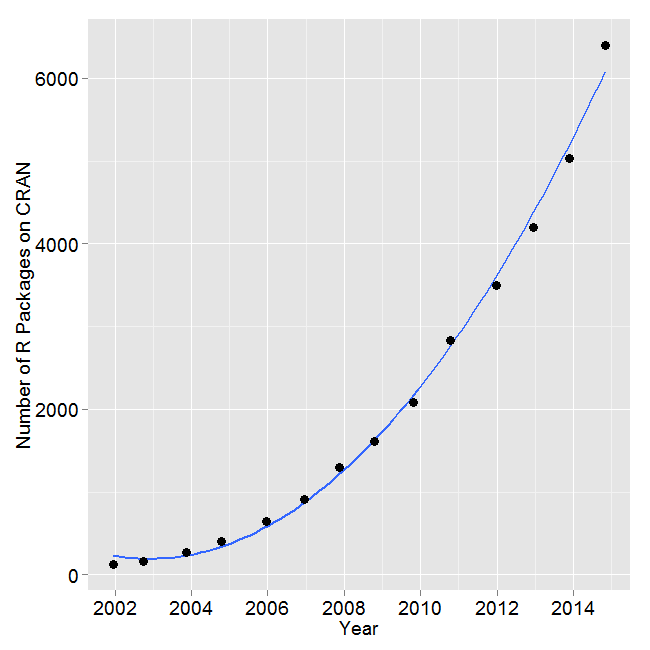
\includegraphics[scale=0.3]{packages}
  \end{frame}

\subsection{Ejercicios para llevar}

\begin{frame}
 \begin{center}
  \Huge \textcolor{blue}{Ejercicios para llevar}
 \end{center}
\end{frame}

\defverbatim[colored]\lst{%
\begin{lstlisting}[language=R,tabsize=8,basicstyle=\ttfamily]

      [,1] [,2] [,3] [,4] [,5]
 [1,]    1   21   41   11   31
 [2,]    3   23   43   13   33
 [3,]    5   25   45   15   35
 [4,]    7   27   47   17   37
 [5,]    9   29   49   19   39
 [6,]   11   31    1   21   41
 [7,]   13   33    3   23   43
 [8,]   15   35    5   25   45
 [9,]   17   37    7   27   47
[10,]   19   39    9   29   49
\end{lstlisting}
}

\begin{frame}
 \frametitle{Ejercicio 1: matrices}
 Cree esta matriz usando una \'unica l\'inea de c\'odigo
\lst
\end{frame}

\defverbatim[colored]\lst{%
\begin{lstlisting}[language=R,tabsize=8,basicstyle=\ttfamily]
<@\textcolor{red}{\# Una solucion:}@>
<@\textcolor{red}{\# crear vector}@>
num <- seq(from=1,to=50,by=2) 
<@\textcolor{red}{\# luego, crear la matriz}@>
matrix(num,nrow=10,ncol=5,byrow=F)

<@\textcolor{red}{\# O, todo en una linea:}@>
matrix(seq(1,50,2),nrow=10,ncol=5,byrow=FALSE)

<@\textcolor{red}{\# que hace el argumento 'byrow=FALSE'?}@>
\end{lstlisting}
}

\begin{frame}
 \frametitle{Soluci\'on 1: matrices}
\lst
\end{frame}

\defverbatim[colored]\lst{%
\begin{lstlisting}[language=R,tabsize=8,basicstyle=\ttfamily]
<@\textcolor{red}{\#1. Cree esta data frame:}@>
cuest num nacimiento  altura  peso    sexo
13     1  13/09/1989  174     66.1    "f"
13     4  05/08/1988  154     60.5    "f"
12     5  06/12/2000  130     110.3   "f"
11     1  08/08/1988  160     156.1   "m"
14     9  04/09/1999  136.6   134.7   "m"
14     1  01/06/2016  NA      NA      "m"
<@\textcolor{red}{\#2. Cree esta otra data frame:}@>
id     estado_civil
14_9   1
14_1   NA
12_5   NA
13_1   1	          
11_1   0
13_4   1


\end{lstlisting}
}

\begin{frame}
 \frametitle{Ejercicio 2: data frame}
\lst
\end{frame}

\begin{frame}
 \frametitle{Ejercicio 3: data frame}
 \begin{enumerate}
 \item Substituya todas los valores desconocidos por "."
 \item Concatene las columnas 'cuest' y 'num' para crear una nueva columna con un identificador \'unico
 \item Agregue la columna 'estado civil' de la segunda data frame a la primera
  \begin{itemize}
	  \item Cu\'antas columnas tiene la nueva base?  
	  \item Qu\'e clase tiene cada columna? Es la clase adecuada para el tipo de datos que contiene?
  \end{itemize}
  \item El peso de los cuestionarios 11,12 y 14 est\'a en libras; transf\'ormelo a kg
  \item Cree una nueva columna para guardar la raz\'on de la altura al peso ($altura \div peso$) para cada fila
  \item Ordene la base de datos con base en esta nueva columna
  \item Guarde la columna 'nacimiento' como clase 'Date'
 \end{enumerate}
\end{frame}

\defverbatim[colored]\lst{%
\begin{lstlisting}[language=R,tabsize=8,basicstyle=\ttfamily]
w <- c(2, 7, 8)
v <- c("A", "B", "C")
x <- list(w, v),
\end{lstlisting}
}

\begin{frame}
 \frametitle{Ejercicio 4: listas\footnote{tomado de http://www.r-bloggers.com/list-exercises/}}
 Si:
\lst
Qu\'e comando usamos para reemplazar "A" en x por "K"?
\begin{enumerate}
 \item  x[[2]] $<$- "K" 
 \item  x[[2]][1] $<$- "K"
 \item  x[[1]][2] $<$- "K" 
\end{enumerate}
\end{frame}

\section{D\'ia 2}

\begin{frame}
 \begin{center}
  \Huge \textcolor{blue}{D\'ia 2}
 \end{center}
\end{frame}

\subsection{Estructuras de control}
\frame{\tableofcontents[currentsection]}

\defverbatim[colored]\lst{%
\begin{lstlisting}[language=R,tabsize=8,basicstyle=\ttfamily]
if (condicion) {accion1}
else {accion2}
<@\textcolor{red}{\# O bien:}@>
if (condicion1) {accion1}
else if (condicion2) {accion2}
\end{lstlisting}
}

\begin{frame}
 \frametitle{Argumentos condicionales}
Permiten definir acciones basadas en la evaluaci\'on de condiciones l\'ogicas.\\
Hay dos princiales:
      \begin{itemize}
 	    \item \textcolor{red}{if}
	    \item \textcolor{red}{else}
  	   \end{itemize}
Importante! A diferencia de Stata:
      \begin{itemize}
 	    \item El condicional \textcolor{red}{if} solo eval\'ua un argumento a la vez
 	    \item Si la condici\'on contiene m\'as de un argumento, solo se eval\'ua el primero y se imprime una advertencia ('warning')
	    \item Para evaluar m\'ultiples argumentos l\'ogicos, use \textcolor{red}{ifelse}
  	   \end{itemize}
  \textcolor{green}{Sintaxis b\'asica}
\lst
\end{frame}

\defverbatim[colored]\lst{%
\begin{lstlisting}[language=R,tabsize=8,basicstyle=\ttfamily]
<@\textcolor{red}{\# Condicional simple:}@>
 x <- "presente en el hogar"
 if (x == "presente en el hogar") <@\textcolor{red}{\# notar '=='}@>
   print("presente")
 if (x == "ausente del hogar") 
   print("ausente")
 if (x != "presente en el hogar" & 
     x !="ausente del hogar")
   print("desconocido")
 
<@\textcolor{red}{\# Ahora, que pasa si probamos:}@>
num <- 1:10
if (num < 5) print("Numero chico")
\end{lstlisting}
}

\begin{frame}
 \frametitle{Ejemplo}
\lst
\end{frame}

\defverbatim[colored]\lst{%
\begin{lstlisting}[language=R,tabsize=8,basicstyle=\ttfamily]
ifelse(condicion, si, no)
\end{lstlisting}
}

\begin{frame}
 \frametitle{ifelse}
 \begin{itemize}
  \item \textcolor{red}{ifelse} es la forma vectorizada de \textcolor{red}{if}
  \item  Uso: aplicar argumentos condicionales a m\'ultiples elementos de un vector
  \item Similar a condicionales \textcolor{red}{if} \textcolor{red}{else} en Stata
  \item Pueden haber varios condicionales subsumidos
  \item Estructura: si condici\'on se cumple, ejecutar acci\'on1, de lo contrario, acci\'on2
  \item NOTA: Recordar siempre asignar la funci\'on a un objeto para conservar el output
 \end{itemize}
\textcolor{blue}{Sintaxis b\'asica}
\lst
\end{frame}


\defverbatim[colored]\lst{%
\begin{lstlisting}[language=R,tabsize=8,basicstyle=\ttfamily]
<@\textcolor{red}{\# datos espurios:}@>
deptos <- c("JUT","HUE","SM","QTZ","CH","ZAC")
set.seed(42) <@\textcolor{red}{\# que es esto?}@>
reg <- sample(deptos,10000,replace=T)
sexo <- sample(c("m","f"),10000,replace=T)
hacinamiento <- sample(0:1,10000,replace=T)
<@\textcolor{red}{\# recodificar por region: "oriente" o "occidente"}@>
reg<-ifelse(
  reg=="JUT" | reg=="CH" | reg=="ZAC", <@\textcolor{red}{\# cond1}@>
  "oriente",  <@\textcolor{red}{\# accion1}@>
  "occidente" <@\textcolor{red}{\# accion2}@>
  )
  
table(reg)
\end{lstlisting}
}

\begin{frame}
 \frametitle{Ejemplo ifelse}
\lst
\end{frame}

\begin{frame}
 \frametitle{Ejercicio ifelse}
Utilice \textcolor{red}{ifelse} y (\textcolor{red}{table} o \textcolor{red}{sum}) para responder la pregunta:\\
\textcolor{blue}{Hay mayor prevalencia de hacinamiento entre mujeres en oriente que en occidente?}
\end{frame}

\defverbatim[colored]\lst{%
\begin{lstlisting}[language=R,tabsize=8,basicstyle=\ttfamily]
<@\textcolor{red}{\# oriente:}@>
<@\textcolor{red}{\# crear vector logico para identificar mujeres:}@>
fem_or<-ifelse(sexo=="f" & reg=="oriente",T,F)
<@\textcolor{red}{\# conservar solo mujeres:}@>
hac_or <- hacinamiento[fem_or]
sum_or <- sum(hac_or) <@\textcolor{red}{\# casos de hacinamiento}@>
oriente <- sum_or/length(hac_or) <@\textcolor{red}{\# prevalencia}@>
<@\textcolor{red}{\# occidente:}@>
fem_oc<-ifelse(sexo=="f" & reg=="occidente",T,F)
hac_oc <- hacinamiento[fem_oc]
sum_oc <- sum(hac_oc)
occidente <- sum_oc/length(hac_oc)

oriente > occidente <@\textcolor{red}{\# evaluar pregunta}@>
\end{lstlisting}
}

\begin{frame}
 \frametitle{Soluci\'on ejercicio ifelse}
\lst
\end{frame}

\defverbatim[colored]\lst{%
\begin{lstlisting}[language=R,tabsize=8,basicstyle=\ttfamily]
<@\textcolor{red}{\# Sintaxis:}@>
while(condicion logica) {operacion}
<@\textcolor{red}{\# Ejemplo:}@>
anio_actual <- 2016 <@\textcolor{red}{\# Fecha actual}@>
respuesta <- ""  <@\textcolor{red}{\# Por que hay que crear esta var?}@>
while(respuesta != anio_actual) {
print("Te pregunto:")
respuesta <- readline("En que anio estamos? > ")
}
\end{lstlisting}
}

\begin{frame}
 \frametitle{Bucles 'while'}
Ejecuta una operacion mientras una condici\'on sea satisfecha.
      \begin{itemize}
       \item El bucle realizar\'a la operaci\'on en tanto el resultado de evaluar la condici\'on sea \textcolor{blue}{TRUE}      	
 	    \item Bucles infinitos con \textcolor{red}{while(T) {operacion}}
  	   \end{itemize}
  	   \textcolor{blue}{Ejemplo}
\lst
\end{frame}

\defverbatim[colored]\lst{%
\begin{lstlisting}[language=R,tabsize=8,basicstyle=\ttfamily]
 <@\textcolor{red}{\# Como hacerlo utilizando next y break?}@>
foo <- 100
while(foo >50) { <@\textcolor{red}{\# definir condicion}@>
foo <- foo - 1
print(foo)
}
<@\textcolor{red}{\# Como hacerlo utilizando next y break?}@>
\end{lstlisting}
}

\begin{frame}
 \frametitle{Para interrumpir bucles}
      \begin{itemize}
 	    \item \textcolor{blue}{next}
	    \item \textcolor{blue}{break}
  	   \end{itemize}
   \textcolor{blue}{Ejemplo}
   Un bucle que cuente en forma descendente desde 100 y se detenga al llegar a 50.
\lst
\end{frame}

\defverbatim[colored]\lst{%
\begin{lstlisting}[language=R,tabsize=8,basicstyle=\ttfamily]
<@\textcolor{red}{\# Primera alternativa:}@>
foo <- 100
while(T) {
foo <- foo - 1
print(foo)
if (foo <= 50) break <@\textcolor{red}{\# condicion}@>
}
<@\textcolor{red}{\# Segunda alternativa:}@>
foo <- 100
while(T) {
foo <- foo - 1
print(foo)
if (foo > 50) next <@\textcolor{red}{\# notar direccion de '$>$'}@>
print("Fin del bucle") <@\textcolor{red}{\# se imprime una sola vez}@>
break
}
\end{lstlisting}
}

\begin{frame}
 \frametitle{Ejemplo: next, break}
\lst
\end{frame}

\defverbatim[colored]\lst{%
\begin{lstlisting}[language=R,tabsize=8,basicstyle=\ttfamily]
for (v en secuencia) {operacion}
\end{lstlisting}
}

\begin{frame}
 \frametitle{Bucles 'for'}
Estructura de control que permite realizar una operaci\'on iterativamente bajo ciertas condiciones.
\begin{itemize}
 \item Pueden considerarse casos especiales de 'while'
 \item usa operadores '[ ]' para pasar valor  actual del vector de cuenta dentro del bucle
\end{itemize}
   \textcolor{blue}{Sintaxis b\'asica}
\lst
\end{frame}

\defverbatim[colored]\lst{%
\begin{lstlisting}[language=R,tabsize=8,basicstyle=\ttfamily]
<@\textcolor{red}{\# Resultado esperado:}@>
[1] "Hola estela"
[1] "Hola carla"
[1] "Hola pedrina"
[1] "Hola isabela"
[1] "Hola juana"
[1] "Hola herlinda"
[1] "Hola maria"
[1] "Hola clara"
\end{lstlisting}
}

\begin{frame}
 \frametitle{Ejemplo: for}
Instrucciones: imprima las siguientes l\'ineas en la consola de R.
\lst
\end{frame}

\defverbatim[colored]\lst{%
\begin{lstlisting}[language=R,tabsize=8,basicstyle=\ttfamily]
<@\textcolor{red}{\# Una soluci\'on:}@>
<@\textcolor{red}{\# Crear un vector con los nombres para iterar:}@>
nombres <- c("estela","carla","pedrina", 
  "isabela","juana","herlinda","maria","clara")   
<@\textcolor{red}{\# definir el bucle:}@>
for (n in 1:length(nombres)) {
saludo <- paste("Hola", nombres[n]) <@\textcolor{red}{\# Notar [n]}@>
print(saludo)
}
<@\textcolor{red}{\# O, mas compacto:}@>
for (n in 1:length(nombres)) 
  print(paste("Hola", nombres[n]))
\end{lstlisting}
}

\begin{frame}
 \frametitle{Soluci\'on ejemplo: for}
\lst
\end{frame}

\subsection{Funciones}
\frame{\tableofcontents[currentsection]}

\defverbatim[colored]\lst{%
\begin{lstlisting}[language=R,tabsize=8,basicstyle=\ttfamily]
function(entrada) {
operacion
return(salida)
}
\end{lstlisting}
}

\begin{frame}
 \frametitle{Funciones}
Conjunto de operaciones, condicionales, etc. Se caracterizan por:
      \begin{itemize}
 	    \item Recibir una entrada (input) - OPCIONAL
	    \item Realizar una operaci\'on - NECESARIO
	    \item Devolver una salida (output) - OPCIONAL
  	   \end{itemize}
  \textcolor{green}{Sintaxis b\'asica}
\lst
\end{frame}

\defverbatim[colored]\lst{%
\begin{lstlisting}[language=R,tabsize=8,basicstyle=\ttfamily]
 <@\textcolor{red}{\# primero, definir la funcion}@>
 resta_argumentos <- function(x,y) {
 z <- x - y
 return(z)
 }
 resta_argumentos(1,99)  <@\textcolor{red}{\# ejecutar funcion}@>
 [1] -98
  <@\textcolor{red}{\# podemos definir condicionales en la funcion}@>
 resta_positivos <- function(x,y) {
  z <- x - y
  if (z < 0) print("Error: Salida negativa")
  else return(z)
 }
 resta_positivos(1,99)
 [1] "Error: Salida negativa"
\end{lstlisting}
}

\begin{frame}
\frametitle{Funciones}
\textcolor{blue}{Ejemplo}
\lst
\end{frame}

\defverbatim[colored]\lst{%
\begin{lstlisting}[language=R,tabsize=8,basicstyle=\ttfamily]
menor <- function(num) <@\textcolor{red}{\# func. auxiliar 1}@>
  print("Menor de 50")
mayor <- function(num) <@\textcolor{red}{\# func. auxiliar 2}@>
  print("Mayor de 50")
decidir <- function() { <@\textcolor{red}{\# funcion principal}@>
 num <- readline("Escriba valor de 1 a 100 > ")
 num <- as.numeric(num)
 if (num <= 50) menor(num)
 else if (num > 50) mayor(num)
}
decidir() <@\textcolor{red}{\# que pasa al ejecutar funcion?}@>
\end{lstlisting}
}

\begin{frame}
 \frametitle{Funciones subsumidas (embedded)}
      \begin{itemize}
		\item Es posible definir funciones que 'llamen' a otras funciones, 
		\item siempre que no exista recursividad infinita.
  	   \end{itemize}
  \textcolor{blue}{Ejemplo}
\lst
\end{frame}

%fun1 <- function() {
%  fun2()
%}
%fun2 <- function() {
%  fun1()
%}
%fun1()

\defverbatim[colored]\lst{%
\begin{lstlisting}[language=R,tabsize=8,basicstyle=\ttfamily]
 <@\textcolor{red}{\# Primero, definir una funcion sin valor de salida}@>
asignar.valor <- function(valor) {
 x <- valor
}
<@\textcolor{red}{\# Ahora el ejemplo...}@>
asignar.valor(20)
print(x)
<@\textcolor{red}{Error: object 'x' not found}@>
\end{lstlisting}
}

\begin{frame}
 \frametitle{Scoping rules: Lexical scoping}
Dadas las normas de ambientaci\'on de R
      \begin{itemize}
 	    \item Toda variable definida dentro de una funci\'on existe \'unicamente dentro de esa funci\'on (y las funciones que dependan de ella)
 	    \item la \'unica excepci\'on es el objeto indicado en la funcion 'return()'
  	   \end{itemize}
  \textcolor{blue}{Ejemplo}
\lst
\end{frame}

\subsection{Importar y explorar datos}
\frame{\tableofcontents[currentsection]}

\defverbatim[colored]\lst{%
\begin{lstlisting}[language=R,tabsize=8,basicstyle=\ttfamily]
read.csv(file, header = TRUE, sep = ",", 
         stringsAsFactors = TRUE)
read.spss(file, use.value.labels = TRUE, 
          to.data.frame = FALSE, ...)\\
read.dta(file,convert.factors=TRUE,...)
\end{lstlisting}
}

\begin{frame}
 \frametitle{Importar datos}
      \begin{itemize}
 	    \item Mejor formato: .csv
	    \item Para importar de Stata, SPSS hay varios paquetes (foreign, RStata, etc.)
	    \item Recordar asignar datos a un objeto en R para conservar
	    \item Al escribir ruta de archivo (en 'file'), usar / en lugar de \textbackslash
	    \item stringsAsFactors es importante
  	   \end{itemize}
  	   \textcolor{blue}{Sintaxis b\'asica}
\lst
\end{frame}

\defverbatim[colored]\lst{%
\begin{lstlisting}[language=R,tabsize=8,basicstyle=\ttfamily]
<@\textcolor{red}{\# Localizar archivo:}@>
install.packages("utils")
library(utils)
path <- choose.files()
<@\textcolor{red}{\# Abrir archivo:}@>
hogares <- read.spss(path, 
            to.data.frame = T)
<@\textcolor{red}{\# para explorar nuestros datos}@>
str(hogares) <@\textcolor{red}{\# resumen de variables}@>
head(hogares[,1:5]) <@\textcolor{red}{\# Muestra primeras 10 lineas}@>
tail(hogares[,1:5]) <@\textcolor{red}{\# ultimas 10 lineas}@>
nrow(hogares) <@\textcolor{red}{\# numero de filas}@>
ncol(hogares) <@\textcolor{red}{\# numero de columnas}@>
\end{lstlisting}
}

\begin{frame}
 \frametitle{Explorar datos}
Datos estan en: 'Dropbox/curso R/data/ensmi\_h.csv'
\lst
\end{frame}

\defverbatim[colored]\lst{%
\begin{lstlisting}[language=R,tabsize=8,basicstyle=\ttfamily]
<@\textcolor{red}{\# MHALTITUD registra altitud de encuesta}@>
hist(hogares$mhaltitud) <@\textcolor{red}{\# histograma}@>
max(hogares$MHALTITUD) <@\textcolor{red}{\# valor maximo}@>
min(hogares$MHALTITUD) <@\textcolor{red}{\# valor minimo}@>
<@\textcolor{red}{\# Nos interesas altitudes menores a 3000m}@> 
hogares <- hogares[hogares$MHALTITUD < 3000,]
mean(hogares$MHALTITUD) <@\textcolor{red}{\# media de columna}@>
median(hogares$MHALTITUD) <@\textcolor{red}{\# mediana de columna}@>
View(hogares) <@\textcolor{red}{\# abrir en pestania}@>
edit(hogares) <@\textcolor{red}{\# abrir para edicion}@>
\end{lstlisting}
}

\begin{frame}
 \frametitle{Ejemplo: recodificar variable}
\lst
\end{frame}

\defverbatim[colored]\lst{%
\begin{lstlisting}[language=R,tabsize=8,basicstyle=\ttfamily]
nombres<-c("estela","carlos","pedro","isabela", 
           "juan","herlinda","mario","clara")
sexo <- c("f","m","m","f","m","f","m","f")
df <- data.frame(nombres, sexo)
df$id <- 1:length(sexo)
df$riqueza <- sample(1:100, length(sexo))
table(df$sexo) <@\textcolor{red}{\# tabular factores}@>
<@\textcolor{red}{\# mean,median,25th and 75th quartiles,min,max}@>
summary(df) 
<@\textcolor{red}{\# con el paquete Hmisc:}@>
install.packages("Hmisc") 
library(Hmisc)
describe(df)
\end{lstlisting}
}

\begin{frame}
 \frametitle{Tabulaciones y descripci\'on}
\lst
\end{frame}

\subsection{Ejercicios para llevar}

\begin{frame}
 \begin{center}
  \Huge \textcolor{blue}{Ejercicios para llevar}
 \end{center}
\end{frame}

\defverbatim[colored]\lst{%
\begin{lstlisting}[language=R,tabsize=8,basicstyle=\ttfamily]
<@\textcolor{red}{\# Use 'sample' para numeros enteros aleatorios}@>
sample(0:1, 10, replace = T)
[1] 1 1 0 1 1 1 1 0 1 1
\end{lstlisting}
}

\begin{frame}
 \frametitle{Ejercicio 1: for}
Escriba un bucle que
\begin{itemize}
 \item iniciando en 1,
 \item en cada iteraci\'on genere un n\'umero entero aleatorio entre 0 y 100;
 \item en cada iteraci\'on imprima la suma de todos los n\'umeros generados hasta ese momento; y
 \item se interrumpa cuando la suma de todos los n\'umeros aleatorios hasta ese momento exceda 10,000
 \item (puntos extra: que al finalizar el bucle, imprima el n\'umero de iteraciones realizadas)
\end{itemize}
 \lst
\end{frame}

\defverbatim[colored]\lst{%
\begin{lstlisting}[language=R,tabsize=8,basicstyle=\ttfamily]
<@\textcolor{red}{\# Una solucion:}@>

set.seed(42) <@\textcolor{red}{\# que es esto?}@>
suma <- 0
while(suma <= 10000 ) {
  aleatorio <- sample(1:100,1)
  suma <- suma + aleatorio
  print(suma)
}
\end{lstlisting}
}

\begin{frame}
 \frametitle{Soluci\'on 1: for}
\lst
\end{frame}

\defverbatim[colored]\lst{%
\begin{lstlisting}[language=R,tabsize=8,basicstyle=\ttfamily]
set.seed(42)
suma <- 0
iter <- 0
while(T) {
  iter <- iter + 1
  aleatorio <- sample(1:100,1)
  suma <- suma + aleatorio
  print(suma)
  if (suma >= 10000) {
    print(paste("iteraciones:",iter))
    break
  }
}
\end{lstlisting}
}

\begin{frame}
 \frametitle{Soluci\'on 1 (puntos extra): for}
\lst
\end{frame}

\defverbatim[colored]\lst{%
\begin{lstlisting}[language=R,tabsize=8,basicstyle=\ttfamily]
<@\textcolor{red}{\# Dados dos vectores:}@>
nombres<-c("estela","carlos","pedro","isabela", 
 "juan","herlinda","mario","clara")
sexo <- c("f","m","m","f","m","f","m","f")
<@\textcolor{red}{\# Resultado esperado:}@>
[1] "estela - femenino"
[1] "carlos - masculino"
[1] "pedro - masculino"
[1] "isabela - femenino"
[1] "juan - masculino"
[1] "herlinda - femenino"
[1] "mario - masculino"
[1] "clara - femenino"
\end{lstlisting}
}

\begin{frame}
 \frametitle{Ejercicio 2: for}
  \begin{enumerate}
  \item Utilice un bucle 'for' y argumentos condicionales para imprimir el siguiente texto en la consola:
 \end{enumerate}
\lst
\end{frame}

\defverbatim[colored]\lst{%
\begin{lstlisting}[language=R,tabsize=8,basicstyle=\ttfamily]
<@\textcolor{red}{\# Una solucion:}@>

for (n in 1:length(nombres)) {
  if (sexo[n] == "m") etiqueta<-"masculino"
  else if (sexo[n] == "f") etiqueta<-"femenino"
  print(paste(nombres[n], "-",etiqueta))
}
<@\textcolor{red}{\# Esto se puede vectorizar para optimizar}@>
<@\textcolor{red}{\# Y este es el proximo ejercicio...}@>
\end{lstlisting}
}

\begin{frame}
 \frametitle{Soluci\'on 2: : for}
\lst
\end{frame}

\defverbatim[colored]\lst{%
\begin{lstlisting}[language=R,tabsize=8,basicstyle=\ttfamily]
<@\textcolor{green}{\# }@>
\end{lstlisting}
}

\defverbatim[colored]\lst{%
\begin{lstlisting}[language=R,tabsize=8,basicstyle=\ttfamily]
<@\textcolor{red}{\# Resultado esperado:}@>
[1] "estela - femenino"   "carlos - masculino"  
"pedro - masculino"   "isabela - femenino" 
[5] "juan - masculino"    "herlinda - femenino" 
"mario - masculino"   "clara - femenino" 
\end{lstlisting}
}

\begin{frame}
 \frametitle{Ejercicio 3: ifelse}
 \begin{enumerate}
  \item Repita el ejercicio 1 sin usar bucles: 
  \item en cambio, use \textcolor{blue}{ifelse} o alg\'un \textcolor{blue}{operador de asignaci\'on}
  \item Imprima el siguiente texto en la consola (no se preocupe si todo se imprime en una \'unica l\'inea):
 \end{enumerate}
\lst
\end{frame}

\defverbatim[colored]\lst{%
\begin{lstlisting}[language=R,tabsize=8,basicstyle=\ttfamily]
<@\textcolor{red}{\#\# Una soluci\'on}@>

<@\textcolor{red}{\# Crear etiquetas basado en sexo:}@>
etiqueta <- 
    ifelse(sexo == "f", "femenino", "masculino")
<@\textcolor{red}{\# Crear vector para imprimir}@>
res <- paste(nombres, "-", etiqueta)
print(res) <@\textcolor{red}{\# Imprimir vector}@>

\end{lstlisting}
}

\begin{frame}
 \frametitle{Soluci\'on 3: ifelse}
\lst
\end{frame}

\begin{frame}
 \frametitle{Ejercicio 4: funciones}
Instrucciones
      \begin{itemize}
 	    \item Funcion que imprima los primeros 10 valores de la secuencia Fibonacci iniciando con 1:
 	     $$ F_{n} = F_{n-1} + F_{n-2} $$
	    \item Una funci\'on que, dado un vector, imprima la media, desviaci\'on est\'andar, y (puntos extra) la mediana
	     $$ \sigma = \sqrt{1/N\sum\limits_{i=1}^{N}(x_{i} - \mu)^2}  $$
	    \item Una funci\'on que, dada una base de datos y un n\'umero o letra, regrese como valor de salida la base de datos con ese n\'umero o letra substituido por NA.
  	   \end{itemize}
\end{frame}

\section{D\'ia 3}

\begin{frame}
 \begin{center}
  \Huge \textcolor{blue}{D\'ia 3}
 \end{center}
\end{frame}

\subsection{Operaciones vectorizadas}
\frame{\tableofcontents[currentsection]}

\defverbatim[colored]\lst{%
\begin{lstlisting}[language=R,tabsize=8,basicstyle=\ttfamily]
 t <- c(5,2,8)
 s <- c(9,5,1)
 <@\textcolor{red}{\# Es cada elemento en t mayor que su contraparte en n?}@>
 <@\textcolor{red}{\# Solucion1: usar bucle}@>
 for (n in 1:length(t)) 
   print(t[n] > s[n])
<@\textcolor{red}{\# Solucion2: vectorizar operacion}@>
 t > s	  
\end{lstlisting}
}

 \begin{frame}
 \frametitle{Bucles y operaciones vectorizadas}
 Las operaciones vectorizadas aplican una funci\'on a cada elemento de un vector 'simult\'aneamente' sin iterar en cada elemento.
      \begin{itemize}
 	    \item En R, todos los objetos son vectores
 	    \item Cada vector es de una clase espec\'ifica
 	    \item []
  	   \end{itemize}
  	   \textcolor{blue}{Considere la operaci\'on:}
  	   \lst
\end{frame}

\defverbatim[colored]\lst{%
\begin{lstlisting}[language=R,tabsize=8,basicstyle=\ttfamily]
 <@\textcolor{red}{\# Ejemplo1}@>
j <- 1
for (i in 1:10) {
    j[i] = 10
}
 <@\textcolor{red}{\# Ejemplo2}@>
 j <- rep(NA, 10)
for (i in 1:10) {
    j[i] = 10
}
\end{lstlisting}
}

 \begin{frame}
 \frametitle{Asignaci\'on de memoria\footnote{http://www.noamross.net/blog/2014/4/16/vectorization-in-r--why.html}}
\textcolor{blue}{Ejemplo 1}
      \begin{enumerate}
 	    \item Buscar al vector en la memoria
 	    \item Crear vector para acomodar m\a's datos (reasignar memoria)
 	    \item Copiar los datos viejos e insertar nuevos
 	    \item Borrar el vector viejo
  	   \end{enumerate}
 \textcolor{blue}{Ejemplo 2 (m\'as veloz)}
 \begin{enumerate}
  \item R no debe reasignar en la memoria a cada iteraci\'on
 \end{enumerate}
  	   \lst
\end{frame}

 \begin{frame}
 \frametitle{Bucles y operaciones vectorizadas\footnote{http://www.noamross.net/blog/2014/4/16/vectorization-in-r--why.html}}
Por qu\'e vectorizar?
      \begin{itemize}
 	    \item Optimizaci\'on
 	    \item Evitar 'efectos secundarios' de bucles
 	    \begin{itemize}
 	     \item for(n in 1:10) print(n)
 	     \item Este loop asigna una variable temporal 'n' al environment actual 
 	     \item Esto puede causar problemas m\'as adelante si se reusa 'n'
 	    \end{itemize}
 	    \item Mantener balance optimizaci\'on-esfuerzo
  	   \end{itemize}
\end{frame}

\defverbatim[colored]\lst{%
\begin{lstlisting}[language=R,tabsize=8,basicstyle=\ttfamily]
nombres <- c("Juana", "Pedrina", "Clara") 
apellido1 <- c("Ixapata", "Osorio", "Sic")
n_completo <- paste(nombres, apellido1) 
n_completo <- paste(n_completo, "Chen")
\end{lstlisting}
}

 \begin{frame}
 \frametitle{C\'omo vectorizar?}
      \begin{itemize}
        \item Pensar en t\'erminos de vectores
 	    \item Evitar usar bucles \textcolor{red}{for} donde sea posible
 	    \item Utilizar \textcolor{red}{ifelse} para aplicar operaciones condicionales a vectores
 	    \item Para vectorizar la aplicacio\'on de una funci\'on a lo largo de un vector, una data frame o una lista, utilizar funciones de la familia \textcolor{red}{apply}
 	  \end{itemize}
 	   \textcolor{blue}{Muchas operaciones se pueden vectorizar!}
 	   \lst
\end{frame}

\defverbatim[colored]\lst{%
\begin{lstlisting}[language=R,tabsize=8,basicstyle=\ttfamily]

setwd("C:/Users/USUARIO/Documents")
hogares2 <- read.csv("hogares.csv")
<@\textcolor{red}{\# mhp15  Fuente de agua para beber.}@>
class(hogares2$MHP15)
levels(hogares2$MHP15)
<@\textcolor{red}{\# crear variable binaria: agua pozo}@>
pozo<-ifelse(
      hogares2$MHP15=="Pozo mecánico/manual", 
      1, 0)
<@\textcolor{red}{\# crear variable binaria: rio o lluvia}@>
prec<-ifelse(hogares2$MHP15=="Agua de lluvia"| 
      hogares2$MHP15=="Río/acequia/manantial", 
      1, 0)
hogares2$prec <- prec <@\textcolor{red}{\# opcional}@>
\end{lstlisting}
}

\begin{frame}
 \frametitle{Ejemplo: Recodificar variables}
datos $>$ hogares.sav
\lst
\end{frame}

\defverbatim[colored]\lst{%
\begin{lstlisting}[language=R,tabsize=8,basicstyle=\ttfamily]
 sapply(X, FUN, ..., simplify = TRUE, 
   USE.NAMES = TRUE)
\end{lstlisting}
}

\begin{frame}
\frametitle{Funciones apply}
Familia de funciones utilizada para aplicar una funci\'on de forma iterativa a una serie de objetos.
      \begin{itemize}
 	    \item \textcolor{red}{apply}: aplica una funci\'on a filas o columnas de matriz (retorna lista, matriz o vector)
	    \item \textcolor{red}{lapply}: aplica una funci\'on a un vector (retorna lista)
	    \item \textbf{\textcolor{red}{sapply}} aplica una funci\'on a un vector (retorna vector o matriz)
	    \item \textcolor{red}{vapply}: similar a sapply, con ciertos par\'ametros predefinidos
  	   \end{itemize}
\lst
\end{frame}


\defverbatim[colored]\lst{%
\begin{lstlisting}[language=R,tabsize=8,basicstyle=\ttfamily]
 id <- 1:10000
 <@\textcolor{red}{\# crear valores aleatorios para las columnas}@>
 riqueza <- runif(10000,min=0.2, max=1)
 nutricion <- runif(10000,min=0.3, max=1)
 distancia <- runif(10000,min=0, max=0.7)
 prevalencia <- runif(10000,min=0, max=1)
 df <- data.frame(id,riqueza,nutricion,
  distancia,prevalencia)
mean(df$riqueza) <@\textcolor{red}{\# media de una columna}@>
<@\textcolor{red}{\# Como calcular la media de cada columna?}@>
\end{lstlisting}
}

\begin{frame}
\frametitle{sapply}
\textcolor{blue}{Ejemplo: calcular media de varias columnas}
\lst
\end{frame}

\defverbatim[colored]\lst{%
\begin{lstlisting}[language=R,tabsize=8,basicstyle=\ttfamily]
sapply(df, mean) <@\textcolor{red}{\# Que nos da esto?}@>
<@\textcolor{red}{\# Otro ejemplo:}@>
<@\textcolor{red}{\# Calcular valor minimo de cada columna mas uno}@>
min_mas_1 <- function(col) {
 val <- min(col) + 1
 val
}
sapply(df, min_mas_1)

\end{lstlisting}
}

\begin{frame}
\frametitle{sapply}
sapply aplica una funci\'on a cada columna de una matriz base de datos

Retorna: vector o matriz
\lst
\end{frame}

\subsection{Aplicaci\'on: estimaciones de desigualdad en R}

\begin{frame}
 \begin{center}
  \Huge \textcolor{blue}{Estimaciones de desigualdad}
 \end{center}
\end{frame}

\begin{frame}
 \frametitle{Plan para c\'alculo de desigualdad}
 \begin{itemize}
  \item Abrir 'curso R/ejercicios/desigualdad.R'
  \item Datos: Enei 2010 en 'curso R/data/enei.sav
  \end{itemize} 
Objetivos:
   \begin{enumerate}
    \item Importar datos a R
    \item Descripci\'on b\'asica de datos
    \item An\'alisis basado en cuantiles 
    \item An\'alisis usando indices de desigualdad
   \end{enumerate}
\end{frame}

% opcion "Weight by..." de SPSS no existe en R

\subsection{Estilo y Depuraci\'on}
\frame{\tableofcontents[currentsection]}

 \begin{frame}
 \frametitle{Estilo}
      \begin{itemize}
 	    \item Tabulaci\'on
 	    \item Cambiar estilo de visualizaci\'on
 	    \item Formato autom\'atico de texto
 	    \item Ocultar bucles
 	    \item Comentar c\'odigo!
  	   \end{itemize}
\end{frame}

\defverbatim[colored]\lst{%
\begin{lstlisting}[language=R,tabsize=8,basicstyle=\ttfamily]
fun <- function(x) x
debug(fun)
\end{lstlisting}
}

\begin{frame}
\frametitle{Depuraci\'on y manejo de errores}
Permite detectar errores en funciones
\begin{itemize}
 \item Es recomendable ubicar errores mediante 'print()'
 \item Si esto no funciona, existe la funcion 'debug()'
\end{itemize}
\textcolor{blue}{Ejemplo}
\lst
\end{frame}

\defverbatim[colored]\lst{%
\begin{lstlisting}[language=R,tabsize=8,basicstyle=\ttfamily]
capitalBelice <- function(){
  while(T) {
    n <- readline("capital de belice? > ")
    if (n != "belmopan") print("No lo creo")
    else if (n == "belmopan") {
      m <- readline("Esta segura/o? (s/n)> ")
      if (m != "s" & m != "n") {
        print("Escriba un valor valido")
      } else if (m == s) {
        print("Muy bien!")
      } else if (m == "n") {
        print("Intente de nuevo.")
      } 
    } 
  } 
}
\end{lstlisting}
}

\begin{frame}
\frametitle{Depure: encuentre el error en la funcion}
\lst
\end{frame}

\subsection{Recursos}

\begin{frame}
 \frametitle{Otros recursos	}
      \begin{itemize}
      \item Documentaci\'on en R (usando '?' en R o en \textcolor{blue}{\href{https://cran.r-project.org/}{CRAN}})
      \item Comunidades de usuarios (\textcolor{blue}{\hyperlink{https://stat.ethz.ch/mailman/listinfo/r-help}{ETHZ}}, \textcolor{blue}{\href{http://stackoverflow.com/}{stackoverflow}}) 
	  \item \textcolor{blue}{\href{http://r-exercises.com/start-here-to-learn-r/}{Ejercicios sobre varios temas}}
      \item Buscador \textcolor{blue}{\href{http://rseek.org/}{rseek}}  o \textcolor{blue}{\href{http://finzi.psych.upenn.edu/search.html}{rsitesearch}}
 	    \item Lista de distribuci\'on de \textcolor{blue}{\href{http://www.r-bloggers.com/}{R-bloggers}}
	    \item Coursera: \textcolor{blue}{\href{https://www.coursera.org/learn/r-programming}{R programming}}
	    \item Para manipulaci\'on de datos: Tutorial de dplyr (\textcolor{blue}{\href{http://www.r-bloggers.com/hadley-wickhams-dplyr-tutorial-at-user-2014-part-1/}{video}})
	    \item Una introducci\'on a la \textcolor{blue}{\href{http://tophcito.blogspot.com/2014/04/social-science-goes-r-weighted-survey.html}{poneraci\'on de datos }} de encuestas usando 'survey' 
	    \item Libros de texto: \textcolor{blue}{\href{http://www.statmethods.net/}{R in Action}}, \textcolor{blue}{\href{http://heather.cs.ucdavis.edu/~matloff/132/NSPpart.pdf}{The Art of R Programming}}, \textcolor{blue}{\href{http://www.cookbook-r.com/}{Cookbook for R}}
  	   \end{itemize}
\end{frame}

\begin{frame}{Tiempo de respuesta en Stackoverflow}
      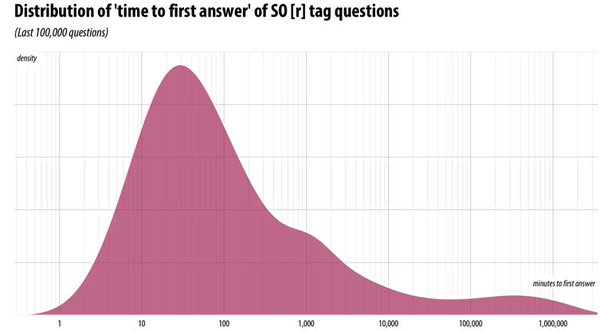
\includegraphics[scale=0.5]{answer}
  \end{frame}

\end{document}

%\defverbatim[colored]\lst{%
%\begin{lstlisting}[language=R,tabsize=8,basicstyle=\ttfamily]
%
%\end{lstlisting}
%}
%
%\begin{frame}
% \frametitle{}
%\lst
%\end{frame}

% Planificacion: Q. 75x modulo
% Dag  25, 2, 9; 
% May: 23, 30, 6
% Horario: 8:30-12:30?
% Lugar: OXFAM? ASIES? 
%
% Para la presentacion:
% MAs ejemplos de la vida real, con bases de datos para que 
% Hablar un poco mas de ponderacion: quiza mostrar un ejemplo de como llegar a un resultado ponderado, pero no meterse al tema en si
